\subsection{Experiment A: Controlled Repeated-Instance Scaling}

\label{subsec:experiment-a}

Experiment A uses four helicopters with equal capacities but different speeds and visual capabilities, serving four demand areas, with 20, 30, 40, 50 and 60 tasks and 30 generated instances per size. Greedy Benefit and Greedy Density are compared with three initializations of the same MILP: cold HiGHS, a Benefit start and a Density start. All methods use the primary-output benefit in Section~3.3. Each MILP treatment receives independent solve allowances of 1, 5, 15, 60 and 600 s. The 600-s runs provide the main comparison; Section~4.3 examines shorter budgets. Allowances are HiGHS parameters, not hard wall-clock deadlines.



At 600 s, cold HiGHS and the Benefit and Density starts certified 150/150, 150/150 and 150/150 instances, respectively. Greedy Benefit had mean paired shortfalls of 12.6--19.1\% across task counts. Greedy Density had mean paired shortfalls of 12.8--16.1\% across task counts.

Every instance has a certified reference. The decline in normalized benefit as task count grows describes the share of mission value served by a fixed fleet; it does not imply a decline in absolute aid delivered. The objective rewards timely weighted output, so completing more tasks alone need not yield greater benefit.


\begin{figure}[!htbp]
\centering
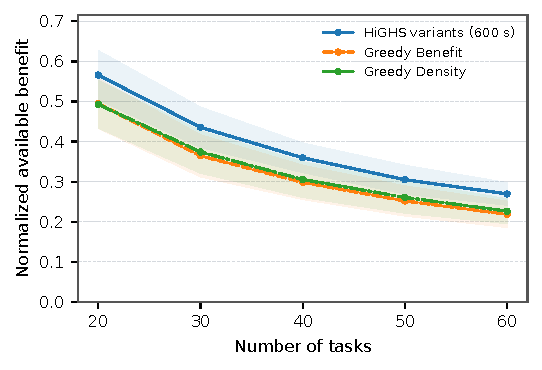
\includegraphics[width=\columnwidth]{A1_solution_quality_coverage_aware.pdf}
\caption{Experiment A benefit at the 600-s MILP allowance. 
Lines show means over the same 30 instances at each task count; bands show
one sample standard deviation. All three MILP variants certified every instance and their paired objective values agree within numerical tolerance, so they are drawn once.}
\label{fig:expA-quality}
\end{figure}


Among matched runs in which both methods certified, median end-to-end time differences relative to cold were HiGHS + Benefit start: +0.03 s (150 pairs); HiGHS + Density start: +0.03 s (150 pairs).

With a 1-s allowance, cold returned incumbents in 2/150 instances, compared with 150/150 and 150/150 for the two starts. This availability largely reflects the supplied constructive plans. Across the shorter allowances, injection improved on cold retaining the same greedy fallback in only 13/1200 paired treatment--budget comparisons (absolute benefit tolerance $10^{-6}$). These repeated comparisons do not represent independent instances. The median injection gain was zero at every budget for each start in this run; the experiment gives no basis for claiming a general search speedup.


\begin{figure*}[!htbp]
\centering
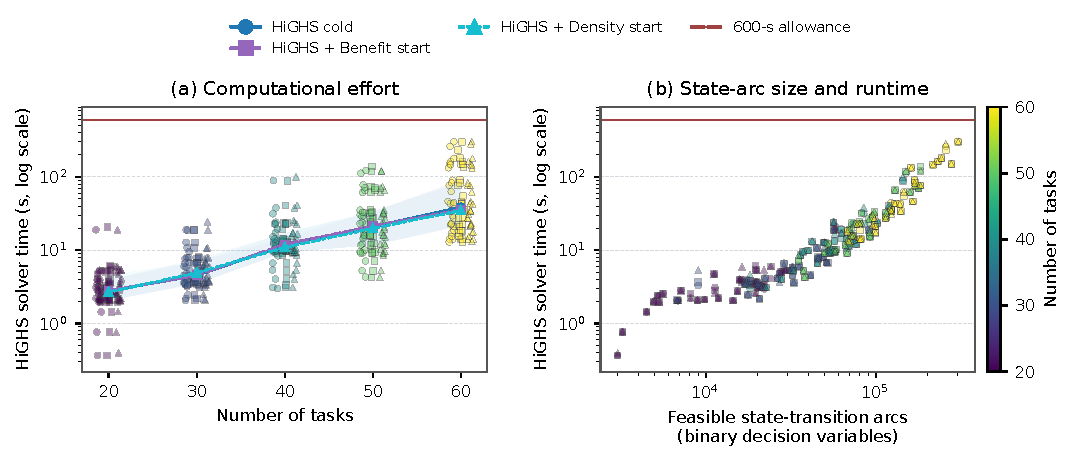
\includegraphics[width=\textwidth]{A8_computational_effort.pdf}
\caption{Experiment A computational effort. Panel (a) shows solver
times with medians and interquartile ranges; panel (b) relates solver time to
generated state-transition arcs. Marker shape identifies the initialization.
Filled markers denote certified runs; open markers, when present, denote
uncertified runs. The dashed line is the 600-s solver allowance.
Table~\ref{tab:expA-runtime} includes preparation time.}
\label{fig:expA-effort}
\end{figure*}


\begin{table}[!htbp]
\centering
\caption{Experiment A: solution quality and certification at the 600-s MILP budget.}
\label{tab:expA-quality}
\scriptsize
\setlength{\tabcolsep}{2.6pt}
\renewcommand{\arraystretch}{1.08}
\begin{tabular}{@{}ccccc@{}}
\toprule
Tasks & \makecell{Normalized available\\benefit\\Mean $\pm$ SD} & \makecell{Completed tasks\\Mean $\pm$ SD} & \makecell{Certified\\runs} & \makecell{Shortfall\\(\%)} \\
\midrule
\multicolumn{5}{@{}l}{\textit{Panel A: HiGHS cold}}\\
\addlinespace[0.2em]
20 & $0.5659 \pm 0.0614$ & $14.40 \pm 1.73$ & $30/30$ & 0.0 \\
30 & $0.4356 \pm 0.0506$ & $16.73 \pm 1.68$ & $30/30$ & 0.0 \\
40 & $0.3595 \pm 0.0371$ & $18.60 \pm 1.71$ & $30/30$ & 0.0 \\
50 & $0.3049 \pm 0.0362$ & $20.07 \pm 2.21$ & $30/30$ & 0.0 \\
60 & $0.2694 \pm 0.0283$ & $20.93 \pm 2.24$ & $30/30$ & 0.0 \\
\midrule
\multicolumn{5}{@{}l}{\textit{Panel B: Greedy Benefit}}\\
\addlinespace[0.2em]
20 & $0.4947 \pm 0.0620$ & $13.67 \pm 1.49$ & -- & 12.6 \\
30 & $0.3643 \pm 0.0527$ & $15.53 \pm 1.78$ & -- & 16.4 \\
40 & $0.2982 \pm 0.0429$ & $16.83 \pm 1.64$ & -- & 17.2 \\
50 & $0.2518 \pm 0.0379$ & $17.77 \pm 1.85$ & -- & 17.6 \\
60 & $0.2184 \pm 0.0331$ & $18.83 \pm 2.25$ & -- & 19.1 \\
\midrule
\multicolumn{5}{@{}l}{\textit{Panel C: Greedy Density}}\\
\addlinespace[0.2em]
20 & $0.4929 \pm 0.0593$ & $13.97 \pm 1.45$ & -- & 12.8 \\
30 & $0.3741 \pm 0.0531$ & $16.30 \pm 1.66$ & -- & 14.2 \\
40 & $0.3053 \pm 0.0447$ & $17.97 \pm 1.79$ & -- & 15.3 \\
50 & $0.2607 \pm 0.0397$ & $19.43 \pm 2.06$ & -- & 14.7 \\
60 & $0.2262 \pm 0.0312$ & $20.47 \pm 2.13$ & -- & 16.1 \\
\midrule
\multicolumn{5}{@{}l}{\textit{Panel D: HiGHS + Benefit start}}\\
\addlinespace[0.2em]
20 & $0.5659 \pm 0.0614$ & $14.40 \pm 1.73$ & $30/30$ & 0.0 \\
30 & $0.4356 \pm 0.0506$ & $16.73 \pm 1.68$ & $30/30$ & 0.0 \\
40 & $0.3595 \pm 0.0371$ & $18.60 \pm 1.71$ & $30/30$ & 0.0 \\
50 & $0.3049 \pm 0.0362$ & $20.07 \pm 2.21$ & $30/30$ & 0.0 \\
60 & $0.2694 \pm 0.0283$ & $20.93 \pm 2.24$ & $30/30$ & 0.0 \\
\midrule
\multicolumn{5}{@{}l}{\textit{Panel E: HiGHS + Density start}}\\
\addlinespace[0.2em]
20 & $0.5659 \pm 0.0614$ & $14.40 \pm 1.73$ & $30/30$ & 0.0 \\
30 & $0.4356 \pm 0.0506$ & $16.73 \pm 1.68$ & $30/30$ & 0.0 \\
40 & $0.3595 \pm 0.0371$ & $18.60 \pm 1.71$ & $30/30$ & 0.0 \\
50 & $0.3049 \pm 0.0362$ & $20.07 \pm 2.21$ & $30/30$ & 0.0 \\
60 & $0.2694 \pm 0.0283$ & $20.93 \pm 2.24$ & $30/30$ & 0.0 \\
\bottomrule
\end{tabular}
\begin{minipage}{0.98\columnwidth}
\footnotesize
Means and sample SD summarize the same instances for all five variants. All MILP variants receive 600 s. Shortfalls are computed per instance against a certified optimum of the same model and objective, then averaged; unknown optima are excluded. Every generated instance has a certified reference. Certification denotes HiGHS optimal status at relative MIP tolerance 1e-06; it is not applicable to the greedy policies.
\end{minipage}
\end{table}


\begin{table}[!htbp]
\centering
\caption{Experiment A: computational performance and generated state-arc MILP size.}
\label{tab:expA-runtime}
\scriptsize
\setlength{\tabcolsep}{2.4pt}
\renewcommand{\arraystretch}{1.08}
\begin{tabular}{@{}ccccc@{}}
\toprule
Tasks & \makecell{Runtime\\Mean $\pm$ SD} & \makecell{Maximum\\runtime} & \makecell{Variables\\mean} & \makecell{Constraints\\mean} \\
\midrule
\multicolumn{5}{@{}l}{\textit{Panel A: HiGHS cold (seconds)}}\\
\addlinespace[0.2em]
20 & $3.52 \pm 3.23$ & $19.28$ & 14{,}939 & 6{,}012 \\
30 & $6.40 \pm 4.39$ & $19.51$ & 32{,}661 & 11{,}697 \\
40 & $16.39 \pm 16.10$ & $90.22$ & 60{,}015 & 18{,}937 \\
50 & $32.22 \pm 30.75$ & $124.10$ & 92{,}362 & 25{,}682 \\
60 & $73.32 \pm 75.90$ & $304.51$ & 144{,}561 & 34{,}880 \\
\midrule
\multicolumn{5}{@{}l}{\textit{Panel B: Greedy Benefit (milliseconds)}}\\
\addlinespace[0.2em]
20 & $1.240 \pm 1.192$ & $7.543$ & -- & -- \\
30 & $1.266 \pm 0.076$ & $1.491$ & -- & -- \\
40 & $1.563 \pm 0.099$ & $1.770$ & -- & -- \\
50 & $1.861 \pm 0.130$ & $2.199$ & -- & -- \\
60 & $2.169 \pm 0.158$ & $2.490$ & -- & -- \\
\midrule
\multicolumn{5}{@{}l}{\textit{Panel C: Greedy Density (milliseconds)}}\\
\addlinespace[0.2em]
20 & $0.870 \pm 0.059$ & $1.097$ & -- & -- \\
30 & $1.143 \pm 0.075$ & $1.334$ & -- & -- \\
40 & $1.484 \pm 0.121$ & $1.752$ & -- & -- \\
50 & $1.759 \pm 0.134$ & $2.035$ & -- & -- \\
60 & $2.136 \pm 0.186$ & $2.495$ & -- & -- \\
\midrule
\multicolumn{5}{@{}l}{\textit{Panel D: HiGHS + Benefit start (seconds)}}\\
\addlinespace[0.2em]
20 & $3.78 \pm 3.55$ & $20.87$ & -- & -- \\
30 & $6.34 \pm 4.35$ & $19.62$ & -- & -- \\
40 & $16.10 \pm 15.96$ & $89.75$ & -- & -- \\
50 & $32.97 \pm 32.97$ & $139.84$ & -- & -- \\
60 & $71.56 \pm 73.48$ & $300.33$ & -- & -- \\
\midrule
\multicolumn{5}{@{}l}{\textit{Panel E: HiGHS + Density start (seconds)}}\\
\addlinespace[0.2em]
20 & $3.73 \pm 3.32$ & $19.32$ & -- & -- \\
30 & $6.48 \pm 4.86$ & $24.62$ & -- & -- \\
40 & $17.12 \pm 18.16$ & $100.76$ & -- & -- \\
50 & $32.23 \pm 31.18$ & $122.60$ & -- & -- \\
60 & $73.07 \pm 78.13$ & $305.27$ & -- & -- \\
\bottomrule
\end{tabular}
\begin{minipage}{0.98\columnwidth}
\footnotesize
End-to-end time includes network and matrix generation, native conversion, model loading and solving. Warm variants additionally include greedy construction, mapping, validation and submission. Preparation is charged to each treatment although shared within the batch. Greedy runtimes are in milliseconds. The common MILP size is reported once. The solver allowance excludes preparation and is not a guaranteed end-to-end deadline.
\end{minipage}
\end{table}

